
\chapter{Current State of Research}

\section{Voice Production System}

\begin{figure} [H]
    \centering
    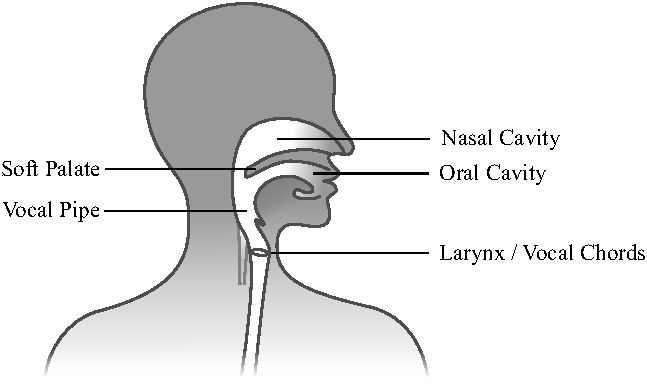
\includegraphics{Graphics/002_VoiceProduction_Physiology.pdf}
    \caption{The human physiology of the organs responsible for the voice production.}
    \label{fig:physiology}
\end{figure}

Early models of the human voice production system were already proposed back in the 1940s \cite{chiba_vowel_1942}. Later on, the source-filter model was widely adopted as a simplified model for the voice production. It was originally proposed in 1960 in \cite{fant_acoustic_1960} but the concept was already explored in experiments with the first vocoder in \cite{dudley_vocoder_1939}, \cite{dudley_remaking_1939}. The source-filter model separates the human voice production in the source and the filter. The source is usually represented by the vocal chords as the organ that initially creates a vibrating air volume, usually referred to as the glottal flow. The filter is represented by vocal tract consisting of the vocal pipe, oral and nasal cavity. The vocal tract filters the glottal flow, creating resonances or formants in the spectrum. \\
There are many ways for a singer to shape the sound. Singers can sing in different registers or phonation modes\cite{sundberg_science_1987} by adjusting the shape of the vocal chords \cite{salomao_what_2009}. The larynx, or voice box, that contains the voice chords, can be moved slightly up and down by singers, shortening or lengthening the vocal tract to alter the filters spectral envelope \cite{sundberg_raised_1976}. By closing the soft palate, singers can decouple the nasal cavity from the remaining vocal tract to again alter the spectral envelope of the filter \cite{elie_characterisation_2009}. Additionally, The singer has control over the filter spectral envelope by shaping the vocal tract, i.e. by moving the tongue or the lips.

\section{Voice Qualities}

In \cite{sundberg_perceptual_1994}, the author classifies voice qualities into timbre, pitch and loudness with timbre qualities being differentiated again in vowel and voice qualities. 
Timbre qualities are mostly controlled by the shape and length vocal tract, and determine the perceived vowel (1st and 2nd formant) and the voice timbre (higher formants). The perceived loudness is not only affected by the overall amplitude but also by the ratio between higher and lower overtone. Temporal variations in pitch, loudness, timbre and phonation are referred to as expression. 

\section{Singing Voice Synthesis}

\begin{figure}[H]
    \centering
    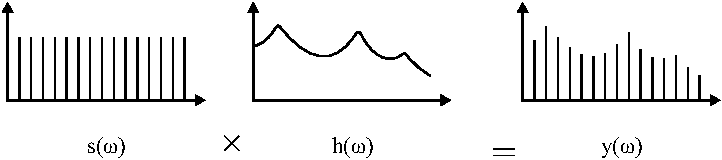
\includegraphics{Graphics/003_SourceFilter_1960.pdf}
    \caption{The source-filter model as proposed in \cite{fant_acoustic_1960}.}
    \label{fig:source_filter}
\end{figure}

Based on early models of the voice production system, some of the first singing voice synthesis methods were source-filter model as described in \cite{fant_acoustic_1960}. The original paper proposes a flat harmonic glottal flow model such as an impulse train as the source $s(\omega)$. The filter $h(\omega)$ could be implemented as an all-pole system that would shaped the vowels formants of the output signal $y(\omega)$ as shown in figure \ref{fig:source_filter}. This model only requires estimation of pitch and the spectral envelope $h(\omega)$. For the purpose of spectral envelope estimation, many methods have been suggested. Linear prediction (LP) was proposed early on \cite{makhoul_linear_1975} with a revised pitch synchronous model (PS LP) proposed in \cite{guerchi_pitch-synchronous_2000}. True Envelope (TE), originally proposed in 1979 \cite{imai_spectral_1979} was rediscovered in 2005 \cite{roebel_efficient_2005}\cite{villavicencio_improving_2006} as one alternative method for spectral envelope estimation. TE iteratively smears the spectrum prior to linear prediction by filtering in the quefreuncy domain to prevent the spectral envelope from overfitting harmonic peaks, an issue commonly seen in LP especially with high pitched signals. More recent methods for spectral envelope estimation include CheapTrick \cite{morise_cheaptrick_2015} or multi frame analysis methods\cite{degottex_simple_2016}.\\

Early on, it was noted that a flat harmonic spectrum is a poor approximation for the glottal flow as the original source-filter model proposed. For that reason, alternative models for the glottal flow, such as the 4-parameter LF model \cite{fant_four-parameter_1985} and the revised 1-parameter LF-$R_d$ model \cite{fant_lf-model_1995} were presented. Source-filter models that see the use of non-flat harmonic signals as the source signal or extend the source-filter model otherwise are usually referred to extended source-filter model. With the introduction of parametric glottal flow models however, the task of separating source and filter is non-trivial. Many methods for source-filter separation were proposed \cite{jinachitra_joint_2005}\cite{degottex_glottal_2010}\cite{perrotin_spectral_2019}. Joint estimation methods provide the means to estimate both source and filter simultaneously. In \cite{loweimi_source-filter_2015}, separation is achieved by analysing trends and fluctuations in the phase domain. Other methods rely on optimization algorithms such as differential evolution \cite{schleusing_joint_2013}.\\

For synthesis of full spoken or sung phrases, concatenative systems \cite{schwarz_concatenative_2006} were proposed. 

\section{Machine Learning in Singign Voice Synthesis}

More recently, machine learning methods for end-to-end singing voice synthesis systems were proposed. These include WaveNet \cite{oord_wavenet:_2016}, an autorregressive neural network that was proposed for the use of text-to-speech or singing voice synthesis. A WaveNet is trained to predict the next sample of an audio sequence and, during generation, uses the predicted sample as it's own input. In \cite{blaauw_neural_2017}, a WaveNet structure was used in conjunction with the WORLD vocoder\cite{morise_world:_2016}. The vocoder extracts spectral envelope coefficients, pitch and an aperiodicity measure from audio and uses the same to recreate the signal. The proposed model uses a modified WaveNet structure to predict the vocoder parameters instead of raw audio. This takes the burden of separating pitch and timbre from the network. As a compromise, any prediction errors in the vocoder analysis or synthesis can't propagate back through the network, resulting in a worse performance than end-to-end approaches \cite{engel_ddsp:_2020}. A similar approach, using Generative Adversarial Networks (GAN) instead of WaveNet for vocoder parameter prediction, is presented in \cite{chandna_wgansing:_2019}. Other approaches include WaveRNN \cite{kalchbrenner_efficient_2018}, based on recurrent neural networks (RNN) and \cite{nakamura_singing_2019}, based on Convolutional Neural Networks.\\

Very recently, differentiable digital signal processing (DDSP) was proposed as a method for combining classical digital signal processing with deep neural networks \cite{engel_ddsp:_2020}. The authors suggested the use of differentiable DSP components such as additive synthesis or FIR filter that could be included in neural networks. The proposed autoencoder architecture uses a decoder to extract pitch, loudness and other latent space control variables from an audio input. The decoder then uses these control variables to predict the coefficients for the DSP components to synthesize the original. Since the dsp components are differentiable, the full architecture can propagate back errors in the synthesized signal and thus can be trained as one network. 


\section{Morphing Singers}

For source-filter models, it was suggested early on that the line spectral frequency (LSF)\cite{itakura_line_1975} representation of all-pole filters shows desirable interpolation characteristics. In \cite{roddy_method_2014} the use of LSF was proposed as a method of morphing between spectral envelopes. 
